\chapter{Additional Information on Congestion-Free Simulation}\label{appendix:additional_info}









\begin{figure}[th]
	\centering
	\begin{subfigure}[b]{0.35\textwidth}
		\centering
		\includegraphics[width=\textwidth]{assets/img/appendix_a/nyc_road_usage_simu2.png}
		\caption{}
		\label{app:fig:nyc_road_usage_simu2}
	\end{subfigure}
	\begin{subfigure}[b]{0.4\textwidth}
		\centering
		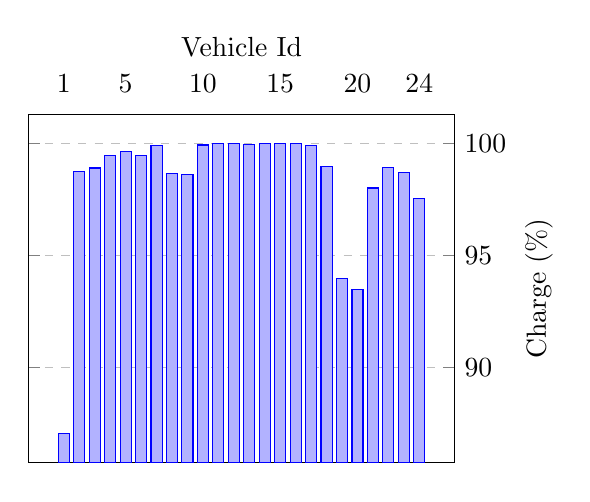
\begin{tikzpicture}
			\begin{axis}[
				ybar,
				xtick=data,
				xtick={1,5, 10,15,20,24},
				xlabel={Vehicle Id},
				ylabel={Charge (\%)},
				bar width=4pt,
				ymajorgrids=true,
				yticklabel pos=right,
				ylabel near ticks,
				grid style=dashed,
				xticklabel pos=right, xlabel near ticks,
				minor x tick num=9,
				xtick style={draw=none},
				width=7cm, 
				height=6cm
				]
				\addplot coordinates{
					(1,87.03273665754057)
					(2,98.75290642116234)
					(3,98.90571811652293)
					(4,99.47446699419078)
					(5,99.660626286003)
					(6,99.45728203892233)
					(7,99.91730734146344)
					(8,98.65314188361312)
					(9,98.59922346939065)
					(10,99.93223998867718)
					(11,100.0)
					(12,100.0)
					(13,99.94747727995325)
					(14,100.0)
					(15,100.0)
					(16,100.0)
					(17,99.92064289494235)
					(18,98.9835856552889)
					(19,93.97807766275497)
					(20,93.47662027131051)
					(21,98.01223510374761)
					(22,98.93486817125883)
					(23,98.71247932045945)
					(24,97.55665230827421)
				};			
			\end{axis}
		\end{tikzpicture}
		\caption{ }
		\label{app:fig:charge_vehicle_baseline_cong_simu2}
	\end{subfigure}
	\caption[Overview of System's Performance with Congestion Limits and Less Charging Time]{Overview of System's Performance without Congestion Limits and Less Charging Time.
		\subfigref{app:fig:nyc_road_usage_simu2} illustrates the utilization of the entire road network during the whole shift, while \subfigref{app:fig:charge_vehicle_baseline_cong_simu2} shows averaging charging percentage of the vehicles. 
	}
	\label{app:fig:nyc_analysis_congestions_simu2}
\end{figure}



\begin{figure}[th]
	\centering
	\begin{subfigure}[b]{0.35\textwidth}
		\centering
		\includegraphics[width=\textwidth]{assets/img/appendix_a/nyc_road_usage_simu5.png}
		\caption{}
		\label{app:fig:nyc_road_usage_simu5}
	\end{subfigure}
	\begin{subfigure}[b]{0.4\textwidth}
		\centering
		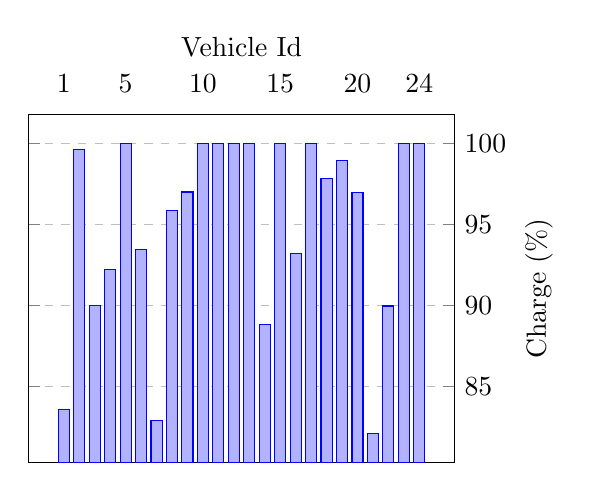
\begin{tikzpicture}
			\begin{axis}[
				ybar,
				xtick=data,
				xtick={1,5, 10,15,20,24},
				xlabel={Vehicle Id},
				ylabel={Charge (\%)},
				bar width=4pt,
				ymajorgrids=true,
				yticklabel pos=right,
				ylabel near ticks,
				grid style=dashed,
				xticklabel pos=right, xlabel near ticks,
				minor x tick num=9,
				xtick style={draw=none},
				width=7cm, 
				height=6cm
				]
				\addplot coordinates{
					(1,83.57186045689065)
					(2,99.6288804845884)
					(3,89.99068368847419)
					(4,92.22928430955479)
					(5,99.97690718579351)
					(6,93.45708118375293)
					(7,82.8937231276273)
					(8,95.87652694720163)
					(9,97.00972201065034)
					(10,100.0)
					(11,100.0)
					(12,100.0)
					(13,100.0)
					(14,88.85404415297268)
					(15,100.0)
					(16,93.23279895120118)
					(17,100.0)
					(18,97.81671755783306)
					(19,98.92678548288295)
					(20,96.97519567053847)
					(21,82.11170560198963)
					(22,89.97414085735168)
					(23,100.0)
					(24,100.0)
				};			
			\end{axis}
		\end{tikzpicture}
		\caption{ }
		\label{app:fig:charge_vehicle_baseline_cong_simu5}
	\end{subfigure}
	\caption[Overview of System's Performance with Congestion Limits and Less Charging Time]{Overview of System's Performance without Congestion Limits and Less Charging Time.
		\subfigref{app:fig:nyc_road_usage_simu2} illustrates the utilization of the entire road network during the whole shift, while \subfigref{app:fig:charge_vehicle_baseline_cong_simu2} shows averaging charging percentage of the vehicles. 
	}
	\label{app:fig:nyc_analysis_congestions_simu5}
\end{figure}






	\begin{figure}
		\begin{tikzpicture}
			\begin{axis}[
				xlabel={Iteration},
				%ylabel={Charge (\%)},
				xtick={0,1,2,3,4,5,6,7,8,9},
				ytick={20,35,50,70,85,100},
				%legend pos=north west,
				legend style={at={(1.05,1)},anchor=north west},
				ymajorgrids=true,
				grid style=dashed,
				thick,
				width=7cm
				]
				
				\addplot[color = viridisbluecolor]
				coordinates {
				(0,100.0)
(1,100.0)
(2,100.0)
(3,100.0)
(4,100.0)
(5,100.0)
(6,96.65992436129552)
(7,100.0)
(8,100.0)
(9,85.30054975932255)
				};
				\addplot[color = viridisyellowcolor]
				coordinates {
				(0,100.0)
(1,100.0)
(2,100.0)
(3,90.0761164440697)
(4,72.36715758393342)
(5,82.02357338140166)
(6,100.0)
(7,100.0)
(8,85.5967113765882)
(9,100.0)
				};
				\addplot[color= viridisgreencolor]
				coordinates {
				(0,100.0)
(1,100.0)
(2,88.32023388997223)
(3,100.0)
(4,100.0)
(5,100.0)
(6,83.39423880255124)
(7,91.17426983229112)
(8,100.0)
(9,100.0)
				};
				
				\addplot[color= viridisorangecolor]
				coordinates {
				(0,100.0)
(1,100.0)
(2,100.0)
(3,100.0)
(4,100.0)
(5,100.0)
(6,100.0)
(7,100.0)
(8,100.0)
(9,100.0)
				};
				
				\addplot[ color = viridispurplecolor]
				coordinates {
				(0,100.0)
(1,100.0)
(2,100.0)
(3,100.0)
(4,100.0)
(5,100.0)
(6,100.0)
(7,39.88363385808256)
(8,69.88363385808256)
(9,99.88363385808256)
				};
				
				\legend{1, 3, 7, 14,2}
				

				
			\end{axis}
		\end{tikzpicture}
		\caption{}
		\label{fig:ex_soc_vehicles_simu5}
	\end{figure}
